\question[15]  Kali tiene una escalera de 666 metros de longitud que quiere usar para bajar a su gato de un árbol.
Coloca la base de la escalera a 2 metros de la base del árbol,
como se muestran a continuación en la figura \ref{fig:proverb_pitagoras_06}
\begin{figure}[H]
    \begin{center}
        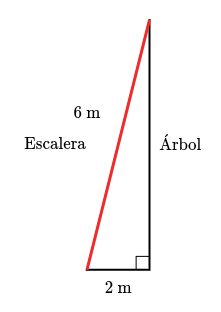
\includegraphics[width=0.3\textwidth]{../images/proverb_pitagoras_06.png}
    \end{center}
    \caption{}
    \label{fig:proverb_pitagoras_06}
\end{figure}
\textbf{¿Qué tan alto en el árbol llegará la escalera?}
\textit{Redondea tu respuesta a la décima de metro más cercana.}